\section{Formal proof structures}
\label{sc:formal}

\def\histx{\hist_\x}
\def\histy{\hist_\y}
\def\histp{\hist_p}
\def\ordlist{L}
\renewcommand{\tleq}{\mathrel{\leq_\ordlist}}
\renewcommand{\tle}{\mathrel{<_\ordlist}}
\renewcommand{\jleq}{\mathrel{\sqsubseteq_\ordlist}}
\newcommand{\E}{E}
\newcommand{\C}{C}
\newcommand{\sx}{S_\x}
\newcommand{\sy}{S_\y}
\newcommand{\spp}{S_p}
\newcommand{\wx}{W_\x}
\newcommand{\wy}{W_\y}
\newcommand{\wpp}{W_p}
\newcommand{\admissible}{\mathsf{fine}}

\paragraph{Specification.}
%
We record a history of the snapshot data structure as a set of entries
of the form $t \mapsto (p, v)$. The entry says that at time $t$ (a
natural number), the value $v$ was written into pointer $p$. Unlike in
the linearizability proof of the snapshot structure, we need to keep
only the write events in the history. The scan events do not modify
the observable by the clients abstract state of the structure, and can
thus be omitted to simplify the considerations.

We keep the following \emph{auxiliary} variables, which are local to
each thread: $\histS$ keeps the finished write events of the
\emph{self} thread, $\histO$ keeps the finished write events of all
other threads, while $\histJ$ keeps the write events that are in
progress. When a call to {\tt write} is initiated, an auxiliary code
will place an appropriate write entry into $\histJ$; when a call
finishes, the entry is moved from $\histJ$ to $\histS$. When one
thread changes its own $\histS$, this immediately changes every other
thread's $\histO$---a discipline provided automatically by FCSL. We
name by $\hist$ the union $\histS \hunion \histO \hunion \histJ$,
which is the history of the overall snapshot data structure. The union
is \emph{disjoint}, as we will enforce an invariant that $\histS$,
$\histO$ and $\histJ$ do not contain timestamps in common.

The timestamps in $\hist$ determine the \emph{real-time} ordering of write
events. We record the \emph{logical} ordering in the auxiliary variable
$\ordlist$. This is a list, storing a permutation of timestamps from
$\hist$. The permutation corresponds to the logical ordering, and we
write $t_1 \tleq t_2$ if $t_1$ appears before $t_2$ in $\ordlist$. In
this sense, $\ordlist$ is the linkage in time for the snapshot
algorithm, and it will be dynamically modified. The ordering $\tleq$
is a total order (i.e., a chain), but as $\tleq$ is dynamic, and thus
subject to change by the algorithm, we introduce further notation and
name by $\jleq$ a \emph{partial suborder} of $\tleq$ that is
stable (i.e., it can only grow over time). We will define $\jleq$ later, but we can already use it to
describe the Hoare triples for {\tt write} and {\tt scan} below. In
fact, it will be important for client reasoning
(Section~\ref{sec:clients}) to keep the definition of $\jleq$ hidden,
so that different snapshot algorithms can provide different
definitions, without influencing the clients.  
%
\begin{equation}
\begin{array}{l}
\mathtt{write}\ (p : \mathtt{ptr}, n : \mathtt{int}) : 
\!\!\!\begin{array}[t]{l}
\{\hists = \hempty \wedge h \subseteq \histO
           \wedge \omega \subseteq {\jleq}\}\\[3pt]
\{\exists t\ldot\, \hists = t \mapsto (p, n) \wedge h \subseteq \histO \wedge
  \omega \subseteq {\jleq}\,{\wedge}\, h \subseteq H^{\hbox{}\sqsubsetneq_\ordlist t}\}
\end{array}\\
%
\mathtt{scan} : 
\!\!\!\begin{array}[t]{l}
\{\hists = \hempty \wedge\, h \subseteq \histO \wedge\,
          \omega \subseteq {\jleq}\}\\[3pt]
\{\hists = \hempty \wedge\, h \subseteq \histO \wedge\, \omega \subseteq {\jleq} \wedge\, \exists\, t\ldot\, %
           h \subseteq H^{\hbox{}\sqsubseteq_\ordlist t} \wedge\,
           \mathsf{chain}\ H^{\hbox{}\sqsubseteq_\ordlist t} \wedge\, r = \mathsf{eval}\ {H^{\hbox{}\sqsubseteq_\ordlist t}}\}
\end{array}
\end{array}
\label{eq:specs}
\end{equation}
%
These are partial correctness Hoare triples, describing how the
program changes the state from the precondition (first braces) to the
postcondition (second braces), possibly influencing the return result
$r$.
%
The expression $H^{\hbox{}\sqsubseteq_\ordlist t}$ selects the entries
in the history $H$ \emph{up to and including} the timestamp $t$,
according to the ordering $\sqsubseteq_\ordlist$. Similarly in
$H^{\hbox{}\sqsubsetneq_\ordlist t}$, except that we exclude $t$.
%

With that in mind, the spec for {\tt write} says the following. We
start with the empty self history indicating that the procedure did
not yet make any writes. We use the variable $h$ to name an arbitrary
subset of the initial value of $\histO$ (hence, of \emph{completed}
write events), and the variable $\omega$ for a subset of the initial
ordering $\jleq$. The postcondition says that when {\tt write}
terminates, one write event $t \mapsto (p, v)$ has finished, and is
hence placed into $\histS$.  $\histO$ and $\jleq$ may have changed
from the previous values, but they still include $h$ and $\omega$ as
subsets. That is, $\histO$ could \emph{only grow}, because other
threads could have created new write events. Similarly for $\jleq$:
other threads could change the ordering in $\ordlist$, but only in a
way which add more relationships between timestamps in
$\jleq$. Lastly, the conjunct
$h \subseteq H^{\hbox{}\sqsubsetneq_\ordlist t}$ says the write events
that have been completed before the call to {\tt write} (and are hence
stored in $h$) will be \emph{ordered before} the event $t$ in
$\sqsubsetneq_\ordlist$. Other threads can permute $L$ to reorder some
entries, but in $L$, $t$ will remain \emph{strictly} after all the
entries from $h$.

The spec for {\tt scan} starts with the same precondition. In the
postcondition, it says that $\histS$ is empty, because {\tt scan}
itself does not execute write events. However, by the time {\tt scan}
returns the pair $r$ as a snapshot, we know that there exists a
timestamp $t$ in the collective history $H$ of the data structure at
which the snapshot \emph{appears} to be taken. First, the conjunct
$h \subseteq H^{\hbox{}\sqsubseteq_\ordlist t}$ indicates that the
snapshot is taken \emph{after} the call to {\tt scan}, because the
finished events stored in $h$ are ordered before (or at best, at)
timestamp $t$. Second, the set $H^{\hbox{}\sqsubseteq_\ordlist t}$ is
a subchain in $\sqsubseteq_\ordlist$ (technically, all its entries are
ordered in $\sqsubseteq_\ordlist$). Intuitively, the chain provides a
way to see how the history logically progressed up to the snapshotting
moment $t$, and moreover, this view will not change in the future in a
way which invalidates $r$ as a snapshot (since $\sqsubseteq_\ordlist$
is stable). Finally, if the chain of writes is evaluated in the order
given by $L$, it produces the snapshot $r$.

\paragraph{Additional auxiliary state.} 
We require yet further structure to describe the admissible ways in
which $\ordlist$ can change while respecting the
specs~(\ref{eq:specs}).

First, we require several variables that will record the code point in
which an executing writer or a scanner currently are. For example, the
auxiliary bits $\sx$ and $\sy$ will be set when the scanner has
cleared the respective forwarding pointer (line~9,
Figure~\ref{fig:jayanti-snapshot}), and reset upon scanner's
termination. Variables $\wx$ and $\wy$ will record the writer state,
and range over the set $\{ \mathsf{Init}, \mathsf{Written}\ t,
\mathsf{Dirty}\ t, \mathsf{Clean}\ t\}$. Here, $t$ is the timestamp we
will logically associate with the write event. $\mathsf{Init}$
indicates that no write is in progress; $\mathsf{Written}\ t$ says
that writer is in line~2 in Figure~\ref{fig:jayanti-snapshot};
$\mathsf{Dirty}\ t$ says that line~3 has finished and $b$ is set
(hence, forwarding in line 5 will occur); $\mathsf{Clean}\ t$ says
that we do not need to track the writer's state anymore, and it is
free to exit.

%
Second, we need to record how events overlap in time. As typical in
linearizability, events that do not overlap will \emph{not} be reordered
wrt.~each other. In the proofs, this is required in order to establish
that the timestamp $t$ in the postcondition of {\tt write} and {\tt
  scan} always appears after the events in $h$. To address this issue,
we keep an auxiliary variable $\E$, storing a function that maps each
timestamp $t$ of a \emph{finished} write events in $\hist$, to a
timestamp identifying the \emph{ending time} of the event.
%
Third, we need to track the visibility of write events with regard to
an ongoing scan method (i.e., is the write missed by the scan). This
will inform how events are reordered in $\ordlist$. We do so by
introducing \emph{colors} for timestamps: $\mathsf{green}$,
$\mathsf{yellow}$ and $\mathsf{red}$. We keep an auxiliary variable
$\C$, storing a function that maps each timestamp in $\hist$ to a
color.
%
The intuition behind the colors is as follows. It is always relative
to the ongoing scan, or the last finished one, if no scans are active.
%
\begin{itemize}
\item Green timestamps identify write events that the scan is
  guaranteed to see. This includes the events that finished before the
  scan started. The order of green timestamps in $\ordlist$ is fixed
  in the following sense: if $\C(t_1) = \mathsf{green}$ and
  $t_1 \tle t_2$, then $t_2$ will never be reordered before $t_1$ in
  $\ordlist$.

\item Yellow timestamps are undecided. The scan may or may not see
  them, hence they may be reorder in $\ordlist$. Due to the
  single-writer/single-scanner assumption, $\hist$ contains at most
  one yellow timestamp per pointer.

\item Red timestamps are guaranteed to be missed by the scan. They
  will be put after the green ones.
\end{itemize}
%
%Color patters turn out to be a very flexible and maleable abstraction
%in order to reasoning about the state of the resource. \gad{I'm
%  looking for a formal way of saying that programming/reasoning about
%  the color lemmas is fun, at least for a FP-minded guy!}

%% In order to prove the correctness of these specs, we introduce the
%% invariants imposed on our axiliary state, as well as the
%% implementation in FCSL of the algorithm, decorated with auxiliary code:

\noindent
%
We can now define $\jleq$ as follows:
\begin{equation}
 t_1 \jleq t_2  = (t_1 = t_2) \vee (E\,(t_1) < t_2) \vee
 (t_1\tle t_2 \wedge \C(t_1) = \mathsf{green}) \label{def-jleq}
\end{equation}
Intuitively, the ordering $t_1 \jleq t_2$ is stable because either the
events associated with $t_1$ and $t_2$ are equal, or non-overlapping,
or $t_1$ is green, and hence fixed, as commented previously.


\paragraph{Invariants}%
The following are (selected) properties relevant to the proof of
specs~\eqref{eq:specs}, that the state (real and auxiliary) of the snapshot
algorithm satisfies throughout execution.  \an{Some are mostly obvious
  book-keeping properties, but some are essential. We should present
  only the important ones.}
\begin{enumerate}

% Self/other histories record finish writes.
\item\label{inv:gapless} $\hist$ is gapless, i.e., contains all the timestamps between
  $0$ and the maximal one. Moreover, each timestamp is associated with
  either the pointer $x$ or the pointer $y$; if we denote by $\histx$
  and $\histy$ the entries in $\hist$ writing into $x$ and $y$
  respectively, then $\hist = \histx \hunion \histy$. \an{removable?}

% Self/other histories record finish writes.
\item\label{inv:finished} $\histS$ and $\histO$ record finished writes: $\dom{E} =
  \dom{\histS \hunion \histO}$. \an{removable?}

% Color invariant
\item\label{inv:color} The colors of the timestamps in $\histx$ and
  $\histy$ can be described by the regular expression $\GYR$. They
  start with a prefix of \emph{at least} one green timestamp, followed
  by \emph{at most} one yellow timestamp, and zero or more reds in the
  tail. Importantly, there is always a (green) entry describing the
  initial write into each $x$ and $y$.
%
%  i.e. the coloring of each of the pointer-view histories satisfies
%  the pattern: many (at least one) green, at most one yellow, zero or
%  more red. \gad{Will I need the refinements?}. This pattern entails
%  that there is an initial value in each of $\histx$ and $\histy$ and,
%  moreover, that initial write is {\bf green}. One of those initial
%  timestamps will be $0$, i.e. $C(0)= green$. In addition, each
%  pointer-view history is sorted in real time -- naturally sorted--
%  and its elements don't overlap.

%% Non-Overlapping are sorted
\item\label{inv:overlap} The ending real time of a finished event
  appears after the initial real time: $\forall\, t \in
  \dom{E}\ldot\ t \leq E(t)$. \an{removable?}  Moreover, events that
  do not overlap in real time are ordered in logical time: $\forall
  t_1 \in \dom{E}, t_2 \in \dom{\hist}$, if $E(t_1) < t_2$ then $t_1
  \tle t_2$.

%% Last keys
\item\label{inv:lastkey} The entry of the last timestamp in $\histx$
  contains the physical value of $\x$: $\x = \histx (\mathsf{last}\,
  \histx)$. Similarly for $y$. \an{removable?}

%% Key Inv for fp
\item\label{inv:forward} If the scanner has cleared $\mathit{fx}$
  ($\sx = \TT$) but a non-$\bot$ value $v$ has been forwarded since
  ($\mathit{fx} = v$), then this is recorded by $\histx$:
  $\exists t\ldot t \mapsto (x, v) \in \histx$. Moreover, $t$ will be
  considered by the scanner, i.e., $t$ is the last green or the yellow
  timestamp in $\histx$. Dually for $\y$.

%  For each $\mathtt{p} \in \{\mathtt{x},\mathtt{y}\}$, if $(S_p \wedge
%  \mathtt{f\_of\ p}= v)$ then exists $t_p$ such that $t_p \hpts (p,v)
%  \in \hist$ and $t_p$ is the last green or yellow timestamp of
%  $\hist_{\mathtt{p}}$ i.e. $t_x = \mathsf{last\_green}\ \histx \vee
%  t_p = \mathsf{yellow\_ts}\ \hist_{\mathtt{p}}$. This property
%  entails that after the scanner has cleared the forwarding pointers,
%  if some new value has been forwarded, its timestamp is the last
%  green or the yellow of the pointer's view-history.

%% Key Inv for p
\item\label{inv:scanner} If the scanner has cleared $\mathit{fx}$
  ($\sx = \TT$), but still has not turned off $\s$ (i.e., it is in
  lines 9-11 in Figure~\ref{fig:jayanti-snapshot}), and $\x = v$ in
  physical state, then this is recorded by $\histx$:
  $\exists t\ldot t \mapsto (x, v) \in \histx$. Moreover, $t$ will be
  considered by the scanner, i.e., $t$ is the last green or the yellow
  timestamp in $\histx$. Dually for $\y$.

%  For each $\mathtt{p} \in \{\mathtt{x},\mathtt{y}\}$, if $(S_p
%  \wedge \mathtt{S})$ then exists $t_p$ such that $t_p \hpts (p,v) \in
%  \hist$ and $t_p$ is, again, the last green or yellow timestamp of
%  $\hist_{\mathtt{p}}$ i.e. $t_x = \mathsf{last\_green}\ \histx \vee
%  t_p = \mathsf{yellow\_ts}\ \hist_{\mathtt{p}}$. This property
%  entails that after the in the scanner has cleared the forwarding
%  pointers and before it unsets the scanner bit {\tt S}, the current
%  value of the pointer was committed by the last green or the yellow
%  timestamp of the pointer's view-history.

%% RedZone invariant
\item\label{inv:redzone} 
%
If $\s = \FF, \sx = \TT, \sy = \TT$, i.e., the scanner is in lines
12-15 in Figure~\ref{fig:jayanti-snapshot}, then $\hist$ satisfies the
$\RZ$ pattern. In other words, if a new write events occur at this
point, it will be colored red, and hence ignored by the scanner.

%If $\wstate{S} = (\FF,\TT,\TT)$ then $\hist$ satisfies the $\RZ$
%coloring pattern: if there is a red timestamp in $\hist$, then then
%the {\sf first} red timestamp partitions $\hist$ so that everything
%before it is yellow or green and everything starting from it is red.
  
\end{enumerate}
%\gad{to do: I'm not sure how deep I should get into the invariants?
%  Won't know for sure until I finish with the proof sketch. We might
%  cut down on them later.}

%\gad{Also: I'm thinking of pushing the invariants down together with
%  the proof sketch, or even fork them together as a separate section
%  sketching the ``correctness'' of our approach}

\begin{figure}
%
\centering
\begin{tabular}{c@{\hfill}c}
%  
\begin{minipage}[t][4cm][t]{.5\textwidth}
\begin{alltt}
\num{1}  write (p, v): () \{
\num{2}   \lat\,\actwrite{p}{v}; \Aux{register}(p,v)\rat;
\num{3}   \lat\,b \tbnd \act{read}(S); \Aux{check}(p,b)\rat;
\num{4}   if b
\num{5}   then \lat\,\actwrite{(f_of p)}{v}; \Aux{forward}(p,b))\rat
\num{6}   else  \lat\,\Aux{finalize}(); return ()\rat\}
\end{alltt}
\end{minipage}
%
&
%
\begin{minipage}[t][4cm][t]{.5\textwidth}
\begin{alltt}
\num{ 7}  scan (): \(A {\times} A\)  \{
\num{ 8}  \lat \actwrite{S}{true}; \Aux{setS}(true)\rat;
\num{ 9}  \lat\,\actwrite{fx}{\(\bot\)}; \Aux{clear}(x)\rat; \lat\,\actwrite{fy}{\(\bot\)}; \Aux{clear}(y)\rat;
\num{10}  vx \tbnd \act{read}(x); vy \tbnd \act{read}(y);
\num{11}  \lat \actwrite{S}{false}; \Aux{setS}(false)\rat;
\num{12}  ox \tbnd \act{read}(fx); oy \tbnd \act{read}(fy);
\num{13}  rx \tbnd if (ox \(\neq\bot\)) then ox else vx;  
\num{14}  ry \tbnd if (oy \(\neq\bot\)) then oy else vy;  
\num{15}  \lat\,\Aux{relink}(rx, ry); return (rx, ry)\,\rat\}
\end{alltt} 
\end{minipage}
%
\end{tabular}
%
\caption{Snapshot procedures annotated with auxiliary code.}
\label{fig:fcsl-snapshot}
\end{figure}


\begin{comment}

I actually want ot be able to implement the code like above, it would
allow us to express better and more precise information about
end-times, and decouple finalize from exit. It would take me a day or
so to do it, but I think it might be worht it.

The correct version should be

\begin{figure}
%
\centering
\begin{tabular}{c@{\hfill}c}
%  
\begin{minipage}[t][4cm][t]{.5\textwidth}
\small
\begin{alltt}
\num{1}  write (p, v): () \{
\num{2}   \lat\,\actwrite{p}{v}; \Aux{register}(p,v)\rat;
\num{3}   \lat\,b \tbnd \act{read}(S); \Aux{check}(p,b)\rat;
\num{4}   if b
\num{5}   then \lat\,\actwrite{(f_of p)}{v}; \Aux{forward}(p,b))\rat
\num{6}   else skip;
\num{7}   \lat\,\Aux{finalize}(); return ()\rat\}
\end{alltt}
\end{minipage}
%
&
%
\begin{minipage}[t][4cm][t]{.5\textwidth}
\small
\begin{alltt}
\num{ 8}  scan (): \(A {\times} A\)  \{
\num{ 9}  \lat \actwrite{S}{true}; \Aux{setS}(true)\rat;
\num{10}  \lat\,\actwrite{fx}{\(\bot\)}; \Aux{clear}(x)\rat; \lat\,\actwrite{fy}{\(\bot\)}; \Aux{clear}(y)\rat;
\num{11}  vx \tbnd \act{read}(x); vy \tbnd \act{read}(y);
\num{12}  \lat \actwrite{S}{false}; \Aux{setS}(false)\rat;
\num{13}  ox \tbnd \act{read}(fx); oy \tbnd \act{read}(fy);
\num{14}  rx \tbnd if (ox \(\neq\bot\)) then ox else vx;  
\num{15}  ry \tbnd if (oy \(\neq\bot\)) then oy else vy;  
\num{16}  \lat\,\Aux{relink}(rx, ry); return (rx, ry)\,\rat\}
\end{alltt} 
\end{minipage}
%
\end{tabular}
%
\caption{Snapshot procedures annotated with auxiliary code.}
\label{fig:fcsl-snapshot}

\end{figure}
\end{comment}


\paragraph{Implementation}%

Figure~\ref{fig:fcsl-snapshot} now presents the annotation of
Jayanti's procedures. We use $\langle$ angle braces $\rangle$ to
enclose a real command with auxiliary code that executes
simultaneously with it.  Note that it is is precisely this auxiliary
procedures that describe how the linearization points of Jayanti's
algorithms are determined, depending on run-time events.
%
As customary in Hoare logic, the auxiliary code is \emph{eraseable};
that is, it only mutates auxiliary variables, but does not modify the
real state. 
%
We name auxiliary code as one would name procedure calls, and proceed
to describe these procedures. Each of them is essentially a
straightforward sequence of reads from some auxiliary variables
followed by assignments of new values to the same variables. Thus
makes it convenient to present each procedures as a Hoare triple,
listing in the precondition the variables read, followed by the newly
assigned values in the postcondition. Unmentioned variables are
considered unchanged.
%
%We present a Hoare-style specification of the auxiliary code so as to
%provide an intuition on how the system evolves. We present the
%auxiliary code transitions as if they act only on parts of the state
%-- e.g. $\wstate{x}$, $\hist$ -- but in fact, they act on the whole
%state of the resource and each of them is required to preserve the
%invariants of the joint state described above. We begin with {\tt
%write}'s auxiliary code:
\[
\begin{array}{l@{\, :\ } l}
%% register
 \aux{register}(p,v) &
  \!\!\! \begin{array}[t]{l}
   \{\ordlist = l,\ \histJ = j,\ \wpp = \mathsf{Init},\, \C = c\}\\ 
   \{\ordlist = \mathsf{snoc}\ l\ t, \histJ = j \hunion t \hpts (p,v), \wpp = \mathsf{Written}\ t,\\
   \phantom{\{} C = \mathsf{if}\ \s \& \spp\ \mathsf{then}\ c[t
                                       \mapsto \mathsf{yellow}]\
                                       \mathsf{else}\ c[t \mapsto \mathsf{red})]\}\quad\mbox{where $t = \mathsf{fresh}\ \hist$}
%c \hunion (t \mapsto \mathsf{if}\ \s \& \spp\ \mathsf{then}\ \mathsf{green}\ \mathsf{else}\ \mathsf{yellow})\}\quad\mbox{where $t = \mathsf{fresh}\ \hist$}
  \end{array} \\[3pt]
%% checkS
 \aux{check}(p,b) & \{\wpp = \mathsf{Written}\, t\}\quad
  \{\wpp = \mathsf{if}\ b\
  \mathsf{then}\ \mathsf{Dirty}\, t\ \mathsf{else}\ \mathsf{Clean}\, t\}\\
%% transfer  
  \aux{forward}(p) &
  \!\!\! \begin{array}[t]{l}
   \{\wpp = \mathsf{Dirty}\, t,\, \C = c \}\\ 
   \{\wpp = \mathsf{Clean}\, t,\, %
   \C= \mathsf{if}\ \s \& \spp\ \mathsf{then}\ c[t \mapsto \mathsf{green}]\ \mathsf{else}\ c\}
  \end{array}\\
%% exit  
  \aux{finalize}(p) &
  \!\!\! \begin{array}[t]{l}
  \{\wpp = \mathsf{Clean}\, t,\ \histS = h,\, %
  \histJ = j \hunion t \hpts (p,v), E = e \}\\
  \{\wpp = \mathsf{Init},\, \histS = h \hunion t \hpts (p,v),\, %
     \histJ = j,\ E = e \hunion t \hpts \mathsf{last}\ \hist \}
 \end{array}
\end{array}
\]
%
%% \[
%% \begin{array}{r c l}
%% %% register
%%  \{\ \hist= h,\ \histJ= j,\ \wstate{p} = \mathsf{Init}\}
%%   & \aux{register}(p,v) &
%%   \{ \!\!\!
%%   \begin{array}[t]{l}
%%    \mathit{let}\ t = \mathsf{fresh}(\hist),\ w = t \hpts (p,v) \\
%%    \mathit{in}\ \histJ= j \hunion w ,\ \wstate{p} = \mathsf{Written}\ t\\
%%    \phantom{\mathit{in}}\ \hist = h \hunion (w,
%%    \mathit{if}\, ({\mathtt S} \wedge S_p)\, \mathit{then}\
%%     \mathbf{yellow}\ \mathit{else}\ \mathbf{red})\}
%%   \end{array}\\
%% %% checkS
%%   \{\ \wstate{p} = \mathsf{Written}\, t\} & \aux{check}(p,b) &
%%   \{\ \wstate{p} = \mathit{if}\ b\
%%   \mathit{then}\ \mathsf{Dirty}\, t\ \mathit{else}\ \mathsf{Clean}\, t\}\\
%% %% transfer  
%%   \{\ \wstate{p} = \mathsf{Dirty}\, t,\ \hist = h\} & \aux{forward}(p) &
%%   \{\!\!\!
%%   \begin{array}[t]{l}
%%    \wstate{p} = \mathsf{Clean}\, t,\\
%%    \hist= \mathit{if}\ ({\mathtt S} \wedge S_p)\,
%%    \mathit{then}\ (\mathsf{paint}\ [t]\ \mathsf{green}\ h)\ \mathit{else}\ h\}
%%   \end{array}\\
%% %% exit  
%%   \{\!\!\! \begin{array}[t]{l}
%%     \wstate{p} = \mathsf{Clean}\, t,\ \histS = h, \\
%%     \histJ = j \hunion t \hpts (p,v), E = e\}
%%   \end{array}\! & \aux{exit}(p) &
%%    \{\!\!\! \begin{array}[t]{l}
%%      \wstate{p} = \mathsf{Init},\ \histS = h \hunion t \hpts (p,v),\\
%%      \histJ = j,\ E = e \hunion t \hpts \mathsf{max}\ \dom{\hist}\}
%%    \end{array}
%% \end{array}
%% \]

%\ifdefined\nosts{}\else%%\usetikzlibrary{arrows,shapes,automata, positioning}
\usetikzlibrary{arrows,shapes,automata,positioning}

%% \begin{figure}[ht]
%% \begin{subfigure}[t]{.4\textwidth}
%% \centering
%% \small
%% \begin{tikzpicture}[->,>=stealth',shorten >=1pt,auto,node distance=3cm,
%%                     thick,initial text={},initial above]
%%   \tikzstyle{every state}=[fill=white,draw,ellipse,text=black]
%%   \node[initial,state] (A)                    {$\mathsf{Init}$};
%%   \node[state]         (B) [below right of=A] {$\mathsf{Written\ t}$};
%%   \node[state]         (D) [below left of=A] {$\mathsf{Clean\ t}$};
%%   \node[state]         (C) [below left of=B] {$\mathsf{Dirty\ t}$};
 
%%   \path (A) edge [bend left]  node {$\act{register}(p,v)$} (B)
%%         (B) edge [bend left]  node {$\act{check}(p,true)$} (C)
%%             edge              node {$\act{check}(p,false)$} (D)
%%         (C) edge [bend left]  node {$\act{forward}(p)$}(D)
%%         (D) edge [bend left]  node {$\act{exit}()$} (A);
%% \end{tikzpicture}
%% \caption{\label{fig:sts:writer} Write STS on $\wstate{p}$}
%% \end{subfigure}%
%% \begin{subfigure}[t]{.6\textwidth}
%% \centering
%% \small
%% \begin{tikzpicture}[->,>=stealth',shorten >=1pt,auto,node distance=2.2cm,
%%                     thick,initial text={},]
%%   \tikzstyle{every state}=[fill=white,draw,ellipse,text=black]
%%   \node[initial,state] (A)                     {$(\FF,\FF,\FF)$};
%%   \node[state]         (B)  [above right of=A] {$(\TT,\FF,\FF)$};
%%   \node[state]         (C1) [above right of=B] {$(\TT,\TT,\FF)$};
%%   \node[state]         (C2) [below right of=B] {$(\TT,\FF,\TT)$};
%%   \node[state]         (D)  [right=2.5 cm of B]  {$(\TT,\TT,\TT)$};
%%   \node[state]         (E)  [below right=0.5cm and 0.cm of C2]
%%                               {$(\FF,\TT,\TT)$};
%%   \path (A)  edge [bend left]   node {$\act{set}(\TT)$} (B)
%%         (B)  edge [bend left]   node {$\act{clear}(\mathtt{x})$} (C1)
%%              edge [bend right]  node {$\act{clear}(\mathtt{y})$} (C2)
%%         (C1) edge [bend left]   node {$\act{clear}(\mathtt{y})$} (D)
%%         (C2) edge [bend right]  node {$\act{clear}(\mathtt{x})$} (D)
%%         (D)  edge [bend left]   node {$\act{set}(\FF)$} (E)
%%         (E)  edge [bend left]   node {$\act{relink}(rx,ry)$} (A);
%% \end{tikzpicture}
%% \caption{\label{fig:sts:scanner} Scan STS on $\wstate{S}$}
%% \end{subfigure}
%%  \caption{\label{fig:sts} The State Transition System described by auxiliary code}
%% \end{figure}

% I don't need the scanner protocol at all
%\begin{figure}

\begin{figure}
\small
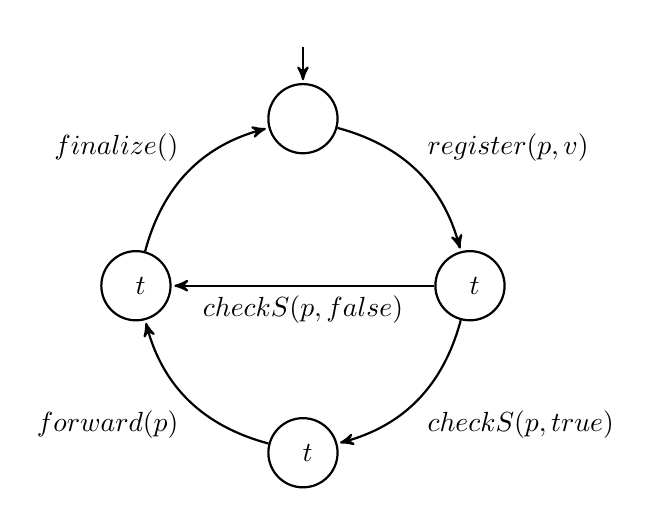
\begin{tikzpicture}[->,>=stealth',shorten >=1pt,auto,node distance=3cm,
                    thick,initial text={},initial above]
  \tikzstyle{every state}=[fill=white,draw,ellipse,text=black]
  \node[initial,state] (A)                    {$\wInit$};
  \node[state]         (B) [below right of=A] {$\wWrite\ t$};
  \node[state]         (D) [below left of=A] {$\wClean\ t$};
  \node[state]         (C) [below left of=B] {$\wDirty\ t$};
 
  \path (A) edge [bend left]  node {$\act{register}(p,v)$} (B)
        (B) edge [bend left]  node {$\act{checkS}(p,true)$} (C)
            edge              node {$\act{checkS}(p,false)$} (D)
        (C) edge [bend left]  node {$\act{forward}(p)$}(D)
        (D) edge [bend left]  node {$\act{finalize}()$} (A);
\end{tikzpicture}
\caption{\label{fig:sts-writer} \jywrite's auxiliary code implements a STS on writer states $\wpp$.}
\end{figure}

\begin{figure}
\small
\begin{tikzpicture}[->,>=stealth',shorten >=1pt,auto,node distance=2cm,
                    thick,initial text={},]
  \tikzstyle{every state}=[fill=white,draw,ellipse,text=black]

  \node[] (I) [] {};
  \node[] (X) [above=1.5 cm of I] {}; 
  \node[state]         (B)  [left=0.5 cm of X]  {$(\sOn,\FF,\FF)$};
  \node[state]         (C)  [right=0.5 cm of X] {$(\sOn,\TT,\FF)$};
  \node[initial,state] (A)  [left= 1.5 cm of I] {$(\sOff\ \_,\FF,\FF)$};
  \node[state]         (D)  [right= 1.5 cm of I] {$(\sOn,\TT,\TT)$};
  \node[state]         (E)  [below=1 cm of I] {$(\sOff\ t,\TT,\TT)$};

\path (A)  edge [bend left]   node {$\act{setS}(\esc{true})$} (B)
        (B)  edge [bend left=10]   node {$\act{clear}(\x)$} (C)
        (C)  edge [bend left]  node {$\act{clear}(\y)$} (D)
        (D)  edge [bend left]   node {$\act{set}(\esc{false})$} (E)
        (E)  edge [bend left]   node {$\act{relink}(rx,ry)$} (A);
\end{tikzpicture}

\caption{\label{fig:sts-scan}%
\jyscan's auxiliary code implements a STS on scanner states $(\spp, \sx, \sy)$.}

\end{figure}
\fi
\noindent
%
For example, $\aux{register}(p, v)$ is executed in line~2 in
Figure~\ref{fig:fcsl-snapshot}, together with the writing of $v$ into
$p$. It allocates a fresh timestamp $t = \mathsf{fresh}\ H$ which will
identify this write, and inserts the appropriate entry
$t \mapsto (p, v)$ into $\histJ$. Next $t$ is added to the end of
$\ordlist$, hence, $t$ will logically appear as a last, until and
unless $\ordlist$ is permuted later. The writer state variable $\wpp$
is changed to indicate that writer finished line~2, with a timestamp
$t$ allocated. The color of $t$ is set to yellow if $\s \& \spp$. In
other words, if an active scanner is in lines 7-9, it is not yet
determined if the write event will be seen or missed by that
scanner. Otherwise, $t$ is painted red, and thus either no scanner
exists, or $t$ will definitely be missed.
%
In line~3, $\aux{check}(p,b)$, depending on $b$, marks the current
write as $\mathsf{Dirty}$ (hence, a scan is in progress, and we should
forward the write), or as $\mathsf{Clean}$, and ready to terminate.
%
In line~5, \aux{forward} paints the allocated timestamp green
(since the scanner is active and in the right lines), because the
event, being forwarded, will definitely be seen by the scanner.
%
$\aux{Finalize}$ moves the current write event from the joint
history $\histJ$ to the thread's self history $\histS$, thus
finalizing it. The maximal currently allocated timestamp of $\hist$ is recorded
in $\E$ as the ending time of the event.

\begin{figure}[t]
%
\centering
\begin{tabular}{c@{\hfill}c}
%
\begin{minipage}[t]{.5\textwidth}
\[
\begin{array}{ll}
\num{1}~ & ~~ \esc{write}\ (p,\, v)\ \{\\ 
\num{2}~ & ~~~~~ \lat\,\actwrite{p}{v}; \aux{register}(p,v)\rat;\\
\num{3}~ & ~~~~~ \lat\, b \tbnd \act{read}(S);\ \aux{check}(p,b) \rat;\\
\num{4}~ & ~~~~~ \kw{if}\ b\\
\num{5}~ & ~~~~~ \kw{then}\ \lat\,%
                           \actwrite{\aleksfwdp{p}}{v};\ \aux{forward}(p)\rat; \\
\num{5'}~           & ~~~~ \lat\,\aux{finalize}(p)\rat\}
\end{array}
\]
\end{minipage}
%
&
%
\begin{minipage}[t]{.5\textwidth}
\[
\begin{array}{rl}
\num{6}~  & \esc{scan} () : ( A \times A )~ \{ \\ 
\num{7}~  & ~~~ \lat\,\actwrite{\s}{\esc{true}};\ \aux{set}(\esc{true}) \rat;\\  
\num{8}~  & ~~~ \lat\,\actwrite{\fx}{\bot};\ \aux{clear}(\x)\rat;\\
\num{9}~  & ~~~ \lat\,\actwrite{\fy}{\bot};\ \aux{clear}(\y)\rat;\\
\num{10}~ & ~~~ \var{vx} \tbnd \lat \act{read}(\x) \rat ; \\
\num{11}~ & ~~~ \var{vy} \tbnd \lat \act{read}(\y) \rat;  \\
\num{12}~ & ~~~ \lat\,\actwrite{\s}{\esc{false}};\ \aux{set}(\esc{false})\rat;\\
\num{13}~ & ~~~ \var{ox} \tbnd \lat \act{read}(\fx) \rat;\\
\num{14}~ & ~~~ \var{oy} \tbnd \lat \act{read}(\fy) \rat;\\
\num{15}~ & ~~~ \var{rx} \tbnd \kw{if}\ (\var{ox} \neq\bot)\
                \kw{then}\ \var{ox}\ \kw{else}\ \var{vx};\\
\num{16}~ & ~~~ \var{ry} \tbnd \kw{if}\ (\var{oy} \neq\bot)\
                \kw{then}\ \var{oy}\ \kw{else}\ \var{vy};\\
\num{17~} & ~~~ \lat\,\aux{relink}(\var{rx}, \var{ry});\
                \kw{return}\ (\var{rx}, \var{ry})\,\rat\}
\end{array}
\]
\end{minipage}
%
\end{tabular}
%
\caption{Snapshot procedures annotated with auxiliary code.}
\label{fig:fcsl-snapshot}
\end{figure}




\section{Auxiliary code implementation}
\label{sc:implementation}

%\paragraph*{Implementation}%

Figure~\ref{fig:fcsl-snapshot} annotates Jayanti's procedures with
auxiliary code (typed in \emph{italic}), with $\langle\mbox{angle
braces}\rangle$ denoting that the enclosed real and auxiliary code
execute \emph{simultaneously} (\ie, atomically). The auxiliary code
builds the histories, evolves the sequence $\ordlist$, and updates the
color of various write events, while respecting the invariants from
Section~\ref{sc:formal}. Thus, it is the \emph{constructive} component
of our proofs. Each atomic command in Figure~\ref{fig:fcsl-snapshot}
represents one \emph{transition} of the STS $C$ from
Figure~\ref{fig:specs}.

%
%As customary, auxiliary code is \emph{erasable} at run time; it does
%not mutate the real state.
%
%% We name auxiliary code as one would name procedure calls, and proceed
%% to describe these procedures.
%

The auxiliary code is divided into several procedures, all of which
are sequences of reads followed by updates to auxiliary variables. We
present them as Hoare triples in Figure~\ref{fig:auxcode}, with the
unmentioned state considered unchanged. The bracketed variables
preceding the triples (\eg, $[t, v]$) are logical variables used to
show how the pre-state value of some auxiliary changes in the
post-state. To symbolize that these triples \emph{define} an atomic
command, rather than merely stating the command's properties, we
enclose the pre- and postcondition in angle brackets $\langle
- \rangle$.

%Following are the characteristic cases.

% %%\usetikzlibrary{arrows,shapes,automata, positioning}
\usetikzlibrary{arrows,shapes,automata,positioning}

%% \begin{figure}[ht]
%% \begin{subfigure}[t]{.4\textwidth}
%% \centering
%% \small
%% \begin{tikzpicture}[->,>=stealth',shorten >=1pt,auto,node distance=3cm,
%%                     thick,initial text={},initial above]
%%   \tikzstyle{every state}=[fill=white,draw,ellipse,text=black]
%%   \node[initial,state] (A)                    {$\mathsf{Init}$};
%%   \node[state]         (B) [below right of=A] {$\mathsf{Written\ t}$};
%%   \node[state]         (D) [below left of=A] {$\mathsf{Clean\ t}$};
%%   \node[state]         (C) [below left of=B] {$\mathsf{Dirty\ t}$};
 
%%   \path (A) edge [bend left]  node {$\act{register}(p,v)$} (B)
%%         (B) edge [bend left]  node {$\act{check}(p,true)$} (C)
%%             edge              node {$\act{check}(p,false)$} (D)
%%         (C) edge [bend left]  node {$\act{forward}(p)$}(D)
%%         (D) edge [bend left]  node {$\act{exit}()$} (A);
%% \end{tikzpicture}
%% \caption{\label{fig:sts:writer} Write STS on $\wstate{p}$}
%% \end{subfigure}%
%% \begin{subfigure}[t]{.6\textwidth}
%% \centering
%% \small
%% \begin{tikzpicture}[->,>=stealth',shorten >=1pt,auto,node distance=2.2cm,
%%                     thick,initial text={},]
%%   \tikzstyle{every state}=[fill=white,draw,ellipse,text=black]
%%   \node[initial,state] (A)                     {$(\FF,\FF,\FF)$};
%%   \node[state]         (B)  [above right of=A] {$(\TT,\FF,\FF)$};
%%   \node[state]         (C1) [above right of=B] {$(\TT,\TT,\FF)$};
%%   \node[state]         (C2) [below right of=B] {$(\TT,\FF,\TT)$};
%%   \node[state]         (D)  [right=2.5 cm of B]  {$(\TT,\TT,\TT)$};
%%   \node[state]         (E)  [below right=0.5cm and 0.cm of C2]
%%                               {$(\FF,\TT,\TT)$};
%%   \path (A)  edge [bend left]   node {$\act{set}(\TT)$} (B)
%%         (B)  edge [bend left]   node {$\act{clear}(\mathtt{x})$} (C1)
%%              edge [bend right]  node {$\act{clear}(\mathtt{y})$} (C2)
%%         (C1) edge [bend left]   node {$\act{clear}(\mathtt{y})$} (D)
%%         (C2) edge [bend right]  node {$\act{clear}(\mathtt{x})$} (D)
%%         (D)  edge [bend left]   node {$\act{set}(\FF)$} (E)
%%         (E)  edge [bend left]   node {$\act{relink}(rx,ry)$} (A);
%% \end{tikzpicture}
%% \caption{\label{fig:sts:scanner} Scan STS on $\wstate{S}$}
%% \end{subfigure}
%%  \caption{\label{fig:sts} The State Transition System described by auxiliary code}
%% \end{figure}

% I don't need the scanner protocol at all
%\begin{figure}

\begin{figure}
\small
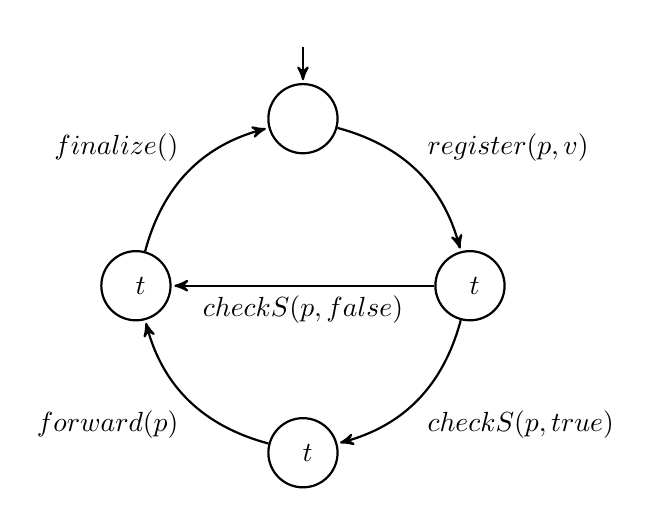
\begin{tikzpicture}[->,>=stealth',shorten >=1pt,auto,node distance=3cm,
                    thick,initial text={},initial above]
  \tikzstyle{every state}=[fill=white,draw,ellipse,text=black]
  \node[initial,state] (A)                    {$\wInit$};
  \node[state]         (B) [below right of=A] {$\wWrite\ t$};
  \node[state]         (D) [below left of=A] {$\wClean\ t$};
  \node[state]         (C) [below left of=B] {$\wDirty\ t$};
 
  \path (A) edge [bend left]  node {$\act{register}(p,v)$} (B)
        (B) edge [bend left]  node {$\act{checkS}(p,true)$} (C)
            edge              node {$\act{checkS}(p,false)$} (D)
        (C) edge [bend left]  node {$\act{forward}(p)$}(D)
        (D) edge [bend left]  node {$\act{finalize}()$} (A);
\end{tikzpicture}
\caption{\label{fig:sts-writer} \jywrite's auxiliary code implements a STS on writer states $\wpp$.}
\end{figure}

\begin{figure}
\small
\begin{tikzpicture}[->,>=stealth',shorten >=1pt,auto,node distance=2cm,
                    thick,initial text={},]
  \tikzstyle{every state}=[fill=white,draw,ellipse,text=black]

  \node[] (I) [] {};
  \node[] (X) [above=1.5 cm of I] {}; 
  \node[state]         (B)  [left=0.5 cm of X]  {$(\sOn,\FF,\FF)$};
  \node[state]         (C)  [right=0.5 cm of X] {$(\sOn,\TT,\FF)$};
  \node[initial,state] (A)  [left= 1.5 cm of I] {$(\sOff\ \_,\FF,\FF)$};
  \node[state]         (D)  [right= 1.5 cm of I] {$(\sOn,\TT,\TT)$};
  \node[state]         (E)  [below=1 cm of I] {$(\sOff\ t,\TT,\TT)$};

\path (A)  edge [bend left]   node {$\act{setS}(\esc{true})$} (B)
        (B)  edge [bend left=10]   node {$\act{clear}(\x)$} (C)
        (C)  edge [bend left]  node {$\act{clear}(\y)$} (D)
        (D)  edge [bend left]   node {$\act{set}(\esc{false})$} (E)
        (E)  edge [bend left]   node {$\act{relink}(rx,ry)$} (A);
\end{tikzpicture}

\caption{\label{fig:sts-scan}%
\jyscan's auxiliary code implements a STS on scanner states $(\spp, \sx, \sy)$.}

\end{figure}



{
%\setlength{\belowcaptionskip}{-5pt}
\begin{figure}[t]
%
\centering
%\begin{subfigure}[t]{1\textwidth}
\small
\[
\begin{array}{l@{\, :\ } l}
%% register
 \aux{register}(p,v) & 
  \begin{array}[t]{l}
   \langle \wpp = \wInit\rangle\\ 
   \langle\ordlistP = \mathsf{snoc}\ {\ordlist}\ t,\
     \histJP = \histJ \hunion t \hpts (p,v),\ \wppP = \wWrite\ t\, v,\\
   \phantom{\langle} \C' = \textrm{if}\ (\sss = \sOn) \& \spp\
                    \textrm{then}\ \C[t \mapsto \mathsf{yellow}]\
                    \textrm{else}\ \C[t \mapsto \mathsf{red}]\rangle \\
   \ \mbox{\small{where $t = \mathsf{fresh}\ \hist = \mathsf{last}\ {\hist}+1$}}
%c \hunion
%(t \mapsto \textrm{if}\ \s \& \spp\ \textrm{then}\ \mathsf{green}\
%\textrm{else}\ \mathsf{yellow})\}\quad\mbox{where $t = \mathsf{fresh}\ \hist$}
  \end{array} \\[2.5pt]
%% checkS
% Im placing it within an  array env so it aligns nicely with the rest
  \aux{check}\,(p,b) & [t, v]\ldot
  \!\begin{array}[t]{l}
  \langle\wpp = \wWrite\ t\, v\rangle\ 
  \langle\wppP = \textrm{if}\ b\
  \textrm{then}\ \wDirty\ t\, \,v\ \textrm{else}\ \wClean\ t\, v\rangle
 \end{array}\\[2.5pt]
%% transfer   
  \aux{forward}\,(p) & [t, v]\ldot
  \!\begin{array}[t]{l}
   \langle\wpp = \wDirty\ t\,v \rangle\\ 
   \langle\wppP = \wClean\ t\,v,\, %
   \C' = \textrm{if}\ (\sss=\sOn) \& \spp\ \textrm{then}\ \C[t \mapsto \mathsf{green}]\ \textrm{else}\ \C\rangle
  \end{array}\\[2.5 pt]
%% exit  
  \aux{finalize}(p) & [t, v]\ldot
  \!\begin{array}[t]{l}
  \langle\wpp = \wClean\ t\, v, %
  t \hpts (p, v) \in \histJ \rangle\\
  \langle\wppP = \wInit,\, \histSP = \histS \hunion t \hpts (p,v),\, %
  \histJP\! = \histJ\setminus\{t\},\,
  \E'\! = \E \hunion\! t \hpts \mathsf{last}\, \hist \rangle
 \end{array}
\end{array}
\]
%\caption{\label{fig:writeauxcode}}
\hrulefill
%\end{subfigure}
%
%\begin{subfigure}[b]{1\textwidth}
\small
\[
\begin{array}{l@{\, :\ }l}
%% setbit
  \aux{set}(b) &
  \begin{array}[t]{l}
        \langle \sss = \textrm{if}\ b\ \textrm{then}\ \sOff\,(\_) \ 
        \textrm{else}\ \sOn,\ \sx = \neg\, b, \sy = \neg\, b \rangle\\
        \langle \sss' = \textrm{if}\ b\ \textrm{then}\ \sOn\ %
        \textrm{else}\ \sOff\,(\mathsf{last}\ \hist),\
         \sx' = \neg\, b, \sy' = \neg\, b \rangle
\end{array}\\[2.5pt] 
%% clear
   \aux{clear}(p) &
  \begin{array}[t]{l}
   \langle\sss = \sOn,\ \spp = \FF \rangle\\
   \langle\sss' = \sOn,\ \spp' = \TT,\
     \CP = \C[\histp \hpts \mathsf{green}] \rangle
  \end{array}\\[2.5pt]
%% re-link
   \aux{relink}(r_x, r_y) & [t_x, t_y]\ldot
    \begin{array}[t]{l}
    \langle\sss = \sOff(\_), %
      t_x \hpts (x, r_x), t_y \hpts (y, r_y) \in \hist, \sx = \sy = \TT, \\
%      \ p \in \{x,y\}:\ \spp =\TT, (t_p = \aux{last\_green}\ \histp \vee
%                \C(t_p) = \mathsf{yellow})\}\\
     \hphantom{\langle} \forall p \in \{x,y\}\ldot \lgVy\ p\, t_p \rangle\\
        \langle\sss' = \sss, \sx'= \sy'=\FF,%
        \CP = \C[t_x, t_y \hpts \mathsf{green}],\\
      \ \ordlist' = \textrm{if}\ (d = \mathsf{Yes}\ x\ s)\
                \textrm{then}\ \aux{push}\ s\ t_y\ \ordlist\\
                 \phantom{\ \ordlist =\ } \textrm{else\ if}\
                 (d = \mathsf{Yes}\ y\ s)\ \textrm{then}\
                 \aux{push}\ s\ t_x\ \ordlist\ \textrm{else}\ \ordlist\rangle\\
  \quad \mbox{where $d = \aux{inspect}\ t_x\, t_y\, \ordlist\, \C$}
  \end{array}
\end{array}
\]
%\caption{\label{fig:scanauxcode}}
%\end{subfigure}
\caption{\label{fig:auxcode} Auxiliary procedures for
%  (\subref{fig:writeauxcode}) 
\jywrite~and 
%(\subref{fig:scanauxcode})
  \jyscan. Bracketed variables (\eg, $[t, v]$) are logical variables
  that scope over precondition and postcondition.}
\end{figure}
}

%\gad{I'm not sure we want to keep the $(t_p =
%  \aux{last\_green}\ \histp \vee \C(t_p) = \mathsf{yellow})$ part, as
%  it is not the pre-variable relating to some auxiliary state
%  projection. This will appear later in the pre and post condition of
%  the atomic commands so it seems repetitive here. Note that the
%  ACTUAL implementation does take a proof that the values are pointed
%  by the last green or yellow timestamp, but there is no need to show
%  that here.}
%
%\gad{In the next section , I'm introducing this as an assertion. So I
%  guess that settles it.}



%The main auxiliary is $\aux{relink}$ in {\tt scan} which decides the
%correctness of snapshot, and whether or not the underlying order
%$\tleq$ has to change. The rest of them are merely doing changes in
%the auxiliary variables in order to provide $\aux{relink}$ with enough
%information to operate. For completeness sake, we will introduce and
%briefly describe all of them, but the reader might consider skipping
%them and go straight down to focus on $\aux{relink}$. We start with
%the auxiliary code for the {\tt write} method, as listed on the first
%column in Figure~\ref{fig:fcsl-snapshot}:
%

%We present a Hoare-style specification of the auxiliary code so as to
%provide an intuition on how the system evolves. We present the
%auxiliary code transitions as if they act only on parts of the state
%-- e.g. $\wstate{x}$, $\hist$ -- but in fact, they act on the whole
%state of the resource and each of them is required to preserve the
%invariants of the joint state described above. We begin with {\tt
%write}'s auxiliary code:


%
%% \[
%% \begin{array}{r c l}
%% %% register
%%  \{\ \hist= h,\ \histJ= j,\ \wstate{p} = \wInit\}
%%   & \aux{register}(p,v) &
%%   \{ \!\!\!
%%   \begin{array}[t]{l}
%%    \mathit{let}\ t = \mathsf{fresh}(\hist),\ w = t \hpts (p,v) \\
%%    \mathit{in}\ \histJ= j \hunion w ,\ \wstate{p} = \wWrite\ t\\
%%    \phantom{\mathit{in}}\ \hist = h \hunion (w,
%%    \mathit{if}\, ({\mathtt S} \wedge S_p)\, \mathit{then}\
%%     \mathbf{yellow}\ \mathit{else}\ \mathbf{red})\}
%%   \end{array}\\
%% %% checkS
%%   \{\ \wstate{p} = \wWrite\, t\} & \aux{check}(p,b) &
%%   \{\ \wstate{p} = \mathit{if}\ b\
%%   \mathit{then}\ \wDirty\, t\ \mathit{else}\ \wClean\, t\}\\
%% %% transfer  
%%   \{\ \wstate{p} = \wDirty\, t,\ \hist = h\} & \aux{forward}(p) &
%%   \{\!\!\!
%%   \begin{array}[t]{l}
%%    \wstate{p} = \wClean\, t,\\
%%    \hist= \mathit{if}\ ({\mathtt S} \wedge S_p)\,
%%    \mathit{then}\ (\mathsf{paint}\ [t]\ \mathsf{green}\ h)\ \mathit{else}\ h\}
%%   \end{array}\\
%% %% exit  
%%   \{\!\!\! \begin{array}[t]{l}
%%     \wstate{p} = \wClean\, t,\ \histS = h, \\
%%     \histJ = j \hunion t \hpts (p,v), E = e\}
%%   \end{array}\! & \aux{exit}(p) &
%%    \{\!\!\! \begin{array}[t]{l}
%%      \wstate{p} = \wInit,\ \histS = h \hunion t \hpts (p,v),\\
%%      \histJ = j,\ E = e \hunion t \hpts \mathsf{max}\ \dom{\hist}\}
%%    \end{array}
%% \end{array}
%% \]

% \gad{TO DO: I updated the writer states to include the $v$ value
% written to memory by an ongoing write event. Figure~\ref{fig:auxcode}
% has been updated but the code below has not!}

%Figure~\ref{fig:sts-writer} presents the intuition for the \jywrite~
%method's auxiliary code, presented as a STS on writer-states.

\paragraph{Auxiliary code for \jywrite.} In line~\lineWrtWrt, $\aux{register}(p, v)$ creates the write event
for the assignment of $v$ to $p$. It allocates a \emph{fresh}
timestamp $t$, inserts the entry $t \mapsto (p, v)$ into $\histJ$, and
adds $t$ to the end of $\ordlist$, thus registering $t$ as the
currently latest write event. The fresh timestamp $t$ is computed out
of the history $\hist$; we take the largest natural number occurring
as a timestamp in $\hist$, and increment it by $1$.  The variable
$\wpp$ updates the writer's state to indicate that the writer finished
line~\lineWrtWrt\ with the timestamp $t$ allocated, and the value $v$
written into $p$. The color of $t$ is set to yellow (\ie, the order
of $t$ is left undetermined), but only if $(\sss= \sOn) \& \spp$
(\ie, an active scanner is in line 10). Otherwise, $t$ is colored
red, indicating that the order of $t$ will be determined by a future
scan.

In line~\lineWrtChk, $\aux{check}(p,b)$, depending on $b$, sets the
writer state to $\wDirty$, indicating that a scan is in progress, and
the writer should forward, or to $\wClean$, indicating that the writer
is ready to terminate.

In line~\lineWrtFwd, \aux{forward} colors the allocated timestamp $t$
green, if an active scanner has passed
lines~\lineScanClearsX--\lineScanClearsY~and is yet to reach
line~\lineScanUnsetsS, because such a scanner will definitely see the
write, either by reading the original value in
lines~\lineScanReadsX--\lineScanReadsY, or by reading the forwarded
value in lines~\lineScanReadsFX--\lineScanReadsFY. Thus, the logical
order of $t$ becomes fixed. In fact, it is possible to derive from the
invariants in Section~\ref{sc:formal}, that this order is the same one
$t$ was assigned at registration, \ie, the linearization point of
this write is line~\lineWrtWrt.

In line~\lineWrtFnz, $\aux{finalize}$ moves the write event $t$ from
the joint history $\histJ$ to the thread's self history $\histS$, thus
acknowledging that $t$ has terminated. The currently largest timestamp
of $\hist$ is recorded in $\E$ as $t$'s ending time. By definition of
$\stableorder$, all the writes that terminated before $t$ in real
time, will be ordered before $t$ in $\stableorder$.

\paragraph{Auxiliary code for \jyscan.} 
%
Method $\aux{set}$ toggles the scanner state $\sss$ on and off. When
executed in line~\lineScanUnsetsS, it returns the timestamp $\toff$
that is currently maximal in real time, as the moment when the scanner
is turned off.
%
%Note that this does not create a fresh timestamp, but rather selects
%that of the last write event in $\hist$.

The procedure $\aux{clear}(p)$ is executed in
lines~\lineScanClearsX--\lineScanClearsY~simultaneously with clearing
the forwarding pointer for $p$. In addition to recording that the
scanner passed lines~\lineScanClearsX\ or
respectively~\lineScanClearsY, by setting the $\spp$ bit, it colors
the subhistory $\histp$ green. Thus, by definition of
$\scanned{\stableorder}$, the ongoing one and all previous writes to
$p$ are recorded as scanned, and thus linearized.

Finally, the key auxiliary procedure of our approach is
$\aux{relink}$. It is executed at line~\lineScanRelinks~just before
the scanner returns the pair $(r_x, r_y)$. Its task is to modify the
logical order of the writes, to make $(r_x, r_y)$ \emph{appear} as a
valid snapshot. This will always be possible under the precondition of
$\aux{relink}$ that the timestamps $t_x$, $t_y$ of the events that
wrote $r_x$, $r_y$ respectively, are either the last green or the
yellow ones in the respective histories $\histx$ and $\histy$, and
$\aux{relink}$ will consider all four cases.  This precondition holds
after line~\lineScanChoosesRY~in Figure~\ref{fig:fcsl-snapshot}, as
one can prove from Invariants~\ref{inv:color} and~\ref{inv:readFP}. In
the precondition we introduce the following abbreviation:
%
\begin{equation}\label{eq:lgVy}
\lgVy\ p\, t\, \eqdef t = \mathsf{last\_green}_{\ordlist}\,
       \histp \vee \C(t) = \mathsf{yellow}
\end{equation}
%% $\lgVy\ {t_p}\ \histp\ \ordlist$ abbreviates $t_p
%% = \mathsf{last\_green}_{\ordlist}\, \histp \vee \C(t_p)
%% = \mathsf{yellow}$.
%% \an{Do we need an abbreviation? The original
%% disjunction seems brief enough?} \gad{Well, not really. I do
%% introduce, however, the abbreviation further down in the atomics'
%% specs.}
%
%Given $(r_x,r_y)$, $\aux{relink}$ does is to identify their timestamps
%$t_x$ and $t_y$. The precondition of $\aux{relink}$ ensures that this
%is either the yellow or--- if there is no such ---the last green
%timestamp in each of $\histx$ and $\histy$. This comes as a result of
%Propositions~\ref{inv:color} and~\ref{inv:readFP} above, amongst
%others.
%%
%% It starts by finding the timestamps $t_x$ and $t_y$ that are
%% responsible for writing $r_x$ and $r_y$ into $\histx$ and $\histy$,
%% respectively. There may be many such timestamps, but we focus on the
%% ones that are yellow, or last green in the respective subhistories of
%% their pointer. It follows from invariants (\ref{inv:forward}) and
%% (\ref{inv:scanner}) that such must exist.


$\aux{Relink}$ uses two helper procedures $\aux{inspect}$ and
$\aux{push}$, to change the logical order. $\aux{Inspect}$ decides if
the selected $t_x$ and $t_y$ determine a valid snapshot, and
$\aux{push}$ performs the actual reordering. The snapshot determined
by $t_x$ and $t_y$ is valid if there is no event $s$ such that
$t_x \tle s \tle t_y$ and $s$ is a write to $x$ (or, symmetrically
$t_y \tle s \tle t_x$, and $s$ is a write to $y$). If such $s$ exists,
$\aux{inspect}$ returns $\mathsf{Yes}\ x\ s$ (or $\mathsf{Yes}\ y\ s$
in the symmetric case). The reordering is completed by $\aux{push}$,
which moves $s$ right after $t_y$ (after $t_x$ in the symmetric case)
in $\tleq$. Finally, $\aux{relink}$ colors $t_x$ and $t_y$ green, to
fix them in $\stableorder$. We can then prove that $(r_x, r_y)$ is a
valid snapshot wrt.~$\stableorder$, and remains so under interference.
%
Notice that the timestamp $s$ returned by $\aux{inspect}$ is always
uniquely determined, and yellow. Indeed, since $t_x$ and $t_y$ are not
red, no timestamp between them can be red either
(Invariant~\ref{inv:redzone}). If $t_x \tle s \tle t_y$ and $s$ is a
write to $x$ (and the other case is symmetric), then $t_x$ must be the
last green in $\histx$, forcing $s$ to be the unique yellow timestamp
in $\histx$, by Invariant~\ref{inv:color}.

%% \gad{ToDo: Remember to add explicit references to Appendix B
%% online.}

%
To illustrate, in Figure~\ref{fig:reorder:before} we have $r_x = 2$,
$r_y = 1$, $t_x$ and $t_y$ are both the last green timestamp of
$\histx$ and $\histy$, respectively, and $t_x \tle t_y$. However,
there is a yellow timestamp $s$ in $\histx$ coming after $t_x$,
encoding a write of $3$. Because $t_x \tle s \tle t_y$, the pair
$(r_x, r_y)$ is not a valid snapshot, thus $\aux{inspect}$ returns
$\mathsf{Yes}\ x\ s$, after which $\aux{push}$ moves $3$ after $1$.

%Next, $\aux{relink}$ uses the helper procedure $\aux{inspect}$ to
%decide if selected $t_x$ and $t_y$ determine a valid snapshot (\ie,
%there are no other events between $t_x$, $t_y$ that make $(r_x, r_y)$
%not be a snapshot).
%
%By way of example, in Figure~\ref{fig:reorder:before} we have $r_x =
%2$, $r_y = 1$, $t_x$ and $t_y$ are both the last green timestamp of
%$\histx$ and $\histy$, respectively, and $t_x \tle t_y$. However,
%there is a yellow timestamp $t'$ in $\histx$ coming after $t_x$,
%encoding a write of $3$. Because $t_x \tle t' \tle t_y$, the pair
%$(r_x, r_y)$ is not a valid snapshot. $\aux{inspect}$ will recognize
%the situation, and indicate to $\aux{relink}$ that $t'$ has to be
%reordered by returning $\mathsf{Yes}\ x\ t'$. The move is completed by
%the helper function $\aux{push}$, which reorders $t'$ right after
%$t_y$ in $\tleq$, as shown in Figure~\ref{fig:reorder:after}.
%Finally, $\aux{relink}$ paints $t_x$ and $t_y$ green, to fix them in
%$\stableorder$. We can then prove that $(r_x, r_y)$ is a valid snapshot
%wrt.~$\stableorder$, and remains so under interference.

% \gad{TO DO: The explanation for relink is still a bit too
% long.}\gad{Do Do I need to explain all auxiliaries? we might consider
% explaining only relink and pushing the rest to the appendices.}


We have omitted the definitions of $\aux{inspect}$ and $\aux{push}$
for the sake of brevity. These are presented in
%
%
\ifdefined\extflag{Appendix~\ref{sc:relink-lemmas}.}
\else {Appendix~B~\cite{CoqFiles}.}
\fi
%
We conclude this section with the main property of $\aux{relink}$,
whose proof can be found in our Coq files~\cite{CoqFiles}.

\begin{lemma}[Main property of $\aux{relink}$]\label{lem:relink-prefix}
Let the precondition of $\aux{relink}$ hold, \ie, $\sss = \sOff(\_)$,
$t_x \hpts (x, r_x), t_y \hpts (y, r_y) \in \hist$, $\sx = \sy =
\TT$, and $\forall p \in \{x,y\}\ldot \lgVy\ p\ t_p$. Then the ending
state of $\aux{relink}$ satisfies the following:
 \begin{enumerate}
 \item\label{lem:relink-lgVy} For all $p \in \{x, y\}$, $t_p =
   \mathsf{last\_green}_{\ordlistP}\, \histp'$.
 \item\label{lem:relink-green} Let $t = \mathsf{max}_{\ordlistP}
   (t_x,t_y)$. Then for every $s \leq_{\ordlistP}t$, $\CP(s) = \mathsf{green}$.
 \end{enumerate}
\end{lemma}



\begin{comment}
%
$\aux{relink}$ works as follows: first, the auxiliary function 
$\mathsf{decide}$ checks $l$ to see if $t_x$ and $t_y$ form a valid 
snapshot, in which case it will return $\mathsf{No}$ and then 
$\ordlist = l$, else it will return $\mathsf{Yes}\ p\ t_r$, indicating 
that there is a miss and that $t_r \in \hist_{p}$--- and is such that 
$t_r \leq t_{\neq p}$ ---should be {\it pushed} in $\ordlist$ past 
$t_{\neq p}$, the latter being $t_y$ if $p=x$, and vice 
versa. Finally, the returned timestamps are painted green.

In Figure~\ref{fig:relink}, we revisit the example from
Section~\ref{sc:overview}, adding the colors to the time-stamps. There
we see in Figure~\ref{fig:relink:before} that $(r_x,ry)$ points to
$(2,1)$ and both timestamps are green. We notice that there is a
yellow in between, $\mathsf{yellow}\, \histx$.  In
Figure~\ref{fig:relink:after}, we see that it has been pushed after
$r_y$.

$\aux{Relink}$ works as follows: first, the auxiliary function 
$\mathsf{decide}$ checks $l$ to see if $t_x$ and $t_y$ form a valid 
snapshot, in which case it will return $\mathsf{No}$ and then 
$\ordlist = l$, else it will return $\mathsf{Yes}\ p\ t_r$, indicating 
that there is a miss and that $t_r \in \hist_{p}$--- and is such that 
$t_r \leq t_{\neq p}$ ---should be {\it pushed} in $\ordlist$ past 
$t_{\neq p}$, the latter being $t_y$ if $p=x$, and vice 
versa. Finally, the returned timestamps are painted green.

We clarify how $\mathsf{decide}$ works: without any loss of
generality, assume $t_x \tleq t_y$. The pre-condition of
$\aux{relink}$ says $t_x$ and $t_y$ are, respectively, the last green
or yellow timestamps of $\histx$ and respectively $\histy$. From the
latter facts facts and Invariant~\ref{inv:redzone}, we know that every
timestamp in the chain from $t_x \tleq t_y$ will be green or yellow
and there will be, at most, two yellow timestamps, one for each
$\histx$ and $\histy$. Then, if $t_x$ is yellow, $\mathsf{decide}$
will return $\mathsf{No}$-- if there are further elements in $\histx$,
they will be in the red tail, and outside the chain-- e.g. the token 7
in Figure~\ref{fig:relink}. Now, if $t_x$ is green and there is no
yellow key in $\histx$, $\mathsf{decide}$ will return
$\mathsf{No}$. If there is, we need to compare it with $t_y$: if
$\mathsf{yellow}\ \histx \tle t_y$, as in Figure~\ref{fig:relink},
$\mathsf{decide}$ will return $\mathsf{Yes}\ x\
(\mathsf{yellow}\, \histx)$ and the latter will be pushed right after
$t_y$ in \ordlist-- $\mathsf{push}$ implements the pointer-swing-like
manipulation on $l$. Last, if $ t_y \tle \mathsf{yellow}\ \histx$
there will be no $\mathsf{push}$ either.

\end{comment}
  


\def\tleqP{\mathrel{\leq_{\ordlist'}}}
\def\tleP{\mathrel{<_{\ordlist'}}}
\def\jleqP{\mathrel{\sqsubseteq_{\ordlist'}}}
%% \subparagraph*{Correctness of write and scan's specifications}%

We devote the rest of the section to illustrating the structure of our
proofs of {\tt write} and {\tt scan}, including aspects of
mechanization in FCSL/Coq. For lack of space, we cannot present the
full theory, but just focus on the structure and a few characteristic
properties.

The first stage of proof (and the mechanization) involves defining the
state space of the algorithm; that is, the definitions of the
auxiliaries, and the invariants that relate them. We presented
selected invariants in Section~\ref{sc:formal}. There is a number of
properties that need to be established under the state space, e.g.,
that it is closed under exchanging history entries between $\histS$
and $\histO$. The latter facilitates dynamic thread creation, because
it allows the reasoning to focus on individual threads in a large
parallel composition.
%
The second stage involves defining the auxiliary code, as in
Figure~\ref{fig:auxcode}, and proving a number of its properties. In
addition to correctness, the properties involve \emph{erasure} (i.e.,
auxiliary code only mutates auxiliary state, but not the real
one), \emph{framing} (i.e., if auxiliary code is executable in some
input heap and input history, then executing it in an extended heap
and history leads to the same results, and the extensions remain
invariant), preservation of invariants (from Section~\ref{sc:formal}),
and \emph{termination}. The correctness aspect of auxiliary code
involves proving that the code preserves the state-space invariants,
and that the precondition and postcondition hold. For example, the
correctness proof of $\aux{relink}$, relies on the following two
helper lemmas.

%The first lemma asserts that $\aux{inspect}$ correctly determines the
%``offending'' timestamp; the second lemma asserts that $\aux{push}$
%modifies the logical ordering in a way that makes the pair $(r_x,
%r_y)$ a valid snapshot.

\begin{lemma}[Correctness of $\aux{inspect}$]\label{lem:inspect}
If $t_x$, $t_y$ are timestamps for write events of $r_x$, $r_y$, then
$\aux{inspect}\ t_x\ t_y\ \ordlist\ \C$ correctly determines that
$(r_x, r_y)$ is a valid snapshot under ordering $\tleq$ and coloring
$C$, or otherwise, returns an ``offending'' timestamp. More formally,
if $\sss = \sOff\ \toff, \sx =\TT, \sy =\TT$, and for each
$p \in \{x,y\}$, $ t_p \hpts (p, r_p) \in \hist$ and $(t_p
= \aux{last\_green}\ \histp \vee \C(t_p) = \mathsf{yellow})$, the
following are exhaustive possibilities.
% if $\aux{inspect}\
%t_x\ t_y\ \ordlist\ \C = \mathsf{No}$ then $(r_x,r_y)$ is a valid
%snapshot. Else, if $\aux{inspect}\ t_x\ t_y\ \ordlist\ \C
%= \mathsf{Yes}\ p\ t'$ then $(r_x,r_y)$ is not a valid snapshot and
%moreover $t'$ is the offending timestamp in $\histp$. Furthermore, by
%exhausting the hypotheses about $t_x$ and $t_y$ we can infer that:
\begin{enumerate}
 \item If $t_x \tle t_y$ and $ \C(t_x) = {\sf yellow}$, then
      $\aux{inspect}\ t_x\ t_y\ \ordlist\ \C
      = \mathsf{No}$. Symmetrically for $t_y \tle t_x$.

 \item If $ t_x \tle t_y $, $ t_x = \aux{last\_green}\ \histx$, and
       $\forall t' \in \histx\ldot\ t_x \tle t'\,{\implies}\,t_y \tle
       t'$, then \\ $\aux{inspect}\ t_x\ t_y\ \ordlist\ \C
       = \mathsf{No}$. Symmetrically for $t_y \tle t_x$.

 \item If $ t_x <_{\ordlist} t_y $, $ t_x = \aux{last\_green}\ \histx
      $, $t' \in \histx$, and $t_x \tle t' \tle t_y$, then
      $\aux{inspect}\ t_x\ t_y\ \ordlist\ \C = \mathsf{Yes}\ \x\ t'$
      and $\C(t') = {\sf yellow}$.  Symmetrically for $t_y \tle t_x$.
\end{enumerate}
\end{lemma}

\begin{lemma}[Correctness of $\aux{push}$]\label{lem:push}
If $\sss = \sOff\ \toff, \sx =\TT, \sy =\TT$, and for $p \in \{x,y\}$,
we have $t_p \hpts (p, r_p) \in \hist$ and $(t_p
= \aux{last\_green}\ \histp \vee \C(t_p) = \mathsf{yellow})$, and
$\aux{inspect}\ t_x\ t_y\ \ordlist\ \C = {\sf Yes}\ p\ t'$, then:
\begin{enumerate}
 \item If $p = x$, then $(r_x, r_y)$ is a valid snapshot under
 $\leq_{\aux{push}\ t'\ t_y\ \ordlist}$. Symmetrically for $p = y$.
\item If $p = x$, then $\ordlist' = \aux{push}\ t'\ t_y\ \ordlist$ and 
$\C' = \C[t_x, t_y \hpts \mathsf{green}]$ satisfy the state space
 invariants
 (Propositions~\ref{inv:overlap}-\ref{inv:redzone}). Symmetrically for
 $p = y$.
\end{enumerate}
\end{lemma}

\begin{comment}
%
%One then has to prove that the state space remains valid under
%exhcanging of history entries between $\histS$ and $\histO$. Such
%exchanging is important because it govens the behavior of auxiliary
%state when threads fork and join, as follows. Let the parent thread be
%$e_1 \parallel e_2$, with \emph{self} history $\histS$
%and \emph{other} history $\histO$.  Upon forking, $\histS$ will be
%split non-deterministically as $\histS = \histS_1 \hunion \histS_2$,
%with $\histS_1$ assigned as a self history of $e_1$, and dually for
%$e_2$. On the other hand, the \emph{other} history of $e_1$ becomes
%$\histO \hunion \histS_2$, to reflect that upon forking $e_2$ becomes
%environment for $e_1$ (and symmetrically for $e_2$).

\subparagraph*{Correctness And Mechanization}%
We finish this section highlighting the most interesting details of
the mechanization of the snapshot data structure in FCSL. Our aim is to
give a general feel of the process of proving a concurrent data
structure correct in the logic, from the definition of the {\it
concurrent resource} for Jayanti's snapshot construction and its
invariants, to the final proof of correctness of the specification of
{\tt write} and {\tt scan} methods from Figure~\ref{fig:specs}. We
will focus mostly on properties of, and assertions about,
$\aux{relink}$ and we refer the reader to Appendix~\ref{sc:coq-code}
and the Coq mechanization~\cite{FCSL:Project} for further detail.

%% \gad{
%% What does an FCSL proof involve:
%% \begin{itemize}
%% \item building the concurrent resource, proving FCSl's meta-theoretic requirements.
%% \item Proving auxiliary code satisfies the invariants i.e. different
%% propositions given before.
%% \item Proving stability of the assertions
%% \item Proving the specs. for the methods
%% \end{itemize}
%% }

% First, build theory for re-linkable histories, auxiliary state,
% invariants and lemmas.

%\gad {Actually, shouldn't we be saying that the proof starts in the
%whitebord?}

The first stage of the mechanization involved building the meta-theory
for re-linkable histories/orders together with the specific auxiliary
state for the snapshot algorithm described above, its properties and
invariants, and several lemmas for reasoning about them. Second, we
implemented the auxiliary code and proved each of them correct,
wrt. to the invariants of the auxiliary code. This entails proving
that each of them satisfies Propositions~\ref{inv:color} --
~\ref{inv:redzone}, among others. We first highlight an intermediate
result about $\aux{inspect}$:

\begin{lemma}[Inspect]\label{lem:inspect}
$\aux{inspect}\ t_x\ t_y\ \ordlist\ \C$ determines if $(r_x, r_y)$ is
a valid snapshot, else finds the \emph{offending} timestamp. More
formally, if $\sss = \sOff\ \toff, \sx =\TT, \sy =\TT$, given $r_x$
and $r_y$ such that for $p \in \{x,y\}$ if $ t_p \hpts (p,
r_p) \in \hist$ and $(t_p = \aux{last\_green}\ \histp \vee \C(t_p)
= \mathsf{yellow}$), then if $\aux{inspect}\ t_x\ t_y\ \ordlist\ \C
= \mathsf{No}$ then $(r_x,r_y)$ is a valid snapshot. Else, if
$\aux{inspect}\ t_x\ t_y\ \ordlist\ \C = \mathsf{Yes}\ p\ t'$ then
$(r_x,r_y)$ is not a valid snapshot and moreover $t'$ is the offending
timestamp in $\histp$. Furthermore, by exhausting the hypotheses about
$t_x$ and $t_y$ we can infer that:
\begin{enumerate}
 \item If $t_x \tle t_y$ and $ \C(t_x) = {\sf yellow}$ then
      $\aux{inspect}\ t_x\ t_y\ \ordlist\ \C = \mathsf{No}$. {\it
      Idem} for $t_x \tle t_y$ and $ \C(t_x) = {\sf yellow})$.

 \item If $ t_x \tle t_y $ and $ t_x = \aux{last\_green}\ \histx $ and
      any timestamp $t'$ that appears after $t_x$ in $\histx $, \ie
      $t_x \tle t' $, also appears after $t_y$ in $\tle$, \ie $
      t_y \tle t' $, then $\aux{inspect}\ t_x\ t_y\ \ordlist\ \C
      = \mathsf{No}$. The same for $ t_y \tle t_x$\ldots, {\it mutatis
      mutandis}.

 \item If $ t_x <_{\ordlist} t_y $ and $ t_x
      = \aux{last\_green}\ \histx $ and there exists a timestamp $t'$
      in $\histx$ such that it appears in $\tleq$ in between $t_x$ and
      $t_y$, \ie $ t_x \tleq t' \tleq t_y $ then $\aux{inspect}\ t_x\
      t_y\ \ordlist\ \C = \mathsf{Yes}\ \x\ t'$. The same for $
      t_y \tle t_x$ \ldots, {\it mutatis mutandis}.
\end{enumerate}
\end{lemma}

%% \begin{lemma}[Inspect]\label{lem:inspect}
%% If $\sss = \sOff\ \toff, \sx =\TT, \sy =\TT$, given $r_x$ and $r_y$
%% such that for $p \in \{x,y\}$ if $ t_p \hpts (p, r_p) \in \hist$ and
%% $(t_p = \aux{last\_green}\ \histp \vee \C(t_p) = \mathsf{yellow}$),
%% then:
%% \begin{enumerate}
%% \item If $(t_x <_{\ordlist} t_y \wedge \C(t_x) = {\sf yellow}) \vee
%%       (t_y <_{\ordlist} t_x \wedge \C(t_y) = {\sf yellow})$ then
%%       $\aux{inspect}\ t_x\ t_y\ \ordlist\ \C = \mathsf{No}$.

%% \item If $ t_x <_{\ordlist} t_y $ and $ t_x
%%       = \aux{last\_green}\ \histx $ and $ \forall\
%%       t' \in \histx\ldot t_x <_{\ordlist} t' \implies t_y <_{\ordlist} t'
%%       $ then $\aux{inspect}\ t_x\ t_y\ \ordlist\ \C
%%       = \mathsf{No}$. Conversely, when $ t_y <_{\ordlist} t_x \ldots
%%       $, {\it mutatis mutandis}.

%% \item If $ t_x <_{\ordlist} t_y $ and $ t_x
%%       = \aux{last\_green}\ \histx $ and $ \exists\ t' \in \histx\ldot
%%       t_x <_{\ordlist} t' <_{\ordlist} t_y $ then $\aux{inspect}\ t_x\
%%       t_y\ \ordlist\ \C = \mathsf{Yes}\ \x\ t'$. Conversely, when $
%%       t_y <_{\ordlist} t_x \ldots $, {\it mutatis mutandis}.
%% \end{enumerate}
%% Moreover, if $\aux{inspect}\ t_x\ t_y\ \ordlist \C = \mathsf{No}$ then
%% $(r_x,r_y)$ is a valid snapshot.
%% \end{lemma}

The lemma above states that $\aux{inspect}$ asserts whether the
timestamps $t_x$ and $t_y$, pointing to the return values $r_x$ and
$r_y$, define a snapshot or not, and in the later case determines the
``offending'' timestamp that needs to be reordered. We consider cases
where $t_x <_{\ordlist} t_y$, as the others are defined conversely. In
the first case, if $t_x <_{\ordlist} t_y$ and $\C(t_x) = {\sf
yellow}$, it follows from $t_y$ being the last green or yellow
timestamp of $\histy$ and Proposition~\ref{inv:redzone} that any
$t' \in \histx$ s.t. $ t_x <_{\ordlist} t'$ will be {\sf red} and
hence $ t_y <_{\ordlist} t'$. Then, $\aux{inspect}\ t_x\
t_y\ \ordlist\ \C = \mathsf{No}$ and $(r_x,r_y)$ will be a valid
snapshot. In the second case, $t_x$ is the last green timestamp of
$\histx$ and, if there is a yellow timestamp $t' \in \histx$ and $ t_y
<_{\ordlist} t'$, then $\aux{inspect}\ t_x\ t_y\ \ordlist\ \C
= \mathsf{No}$, and clearly, $(r_x, r_y)$ is a valid snapshot. In the
last case, there exists a yellow timestamp $t'$ s.t. $ t' <_{\ordlist}
t_y$, so $t'$ invalidates $(r_x, r_y)$ as a snapshot and consequently
$\aux{inspect}\ t_x\ t_y\ \ordlist\ \C = {\sf Yes}\ \x\ t'$, denoting
that $t'$ has to be reordered in $\tle$.
%
%% We refer the reader to the {\tt Coq} mechanization for the formalities
%% of Lemma~\ref{lem:inspect}.
We next prove that, in the later case,
%
%% We next prove that when $\aux{inspect}\ t_x\ t_y\ \ordlist\ \C = {\sf
%% Yes}\ p\ t'$,
the result of $\aux{pushl}\ t'\ t_y\ \ordlist$ fixes the order $\tleq$
such that $(r_x, r_y)$ is a valid snapshot in $\leq_{(\aux{push}\ t'\
t_y\ \ordlist)}$:

\begin{lemma}[Push]\label{lem:push} $\aux{push}\ t'\ t_p$ fixes $\tleq$
so that $(r_x,t_y)$ is a correct snapshot in $\leq_{\aux{push}\ t'\
t_{p}\ \ordlist}$. More formally, if $\sss = \sOff\ \toff, \sx
=\TT, \sy =\TT$, given $r_x$ and $r_y$ such that for $p \in \{x,y\}$
if $ t_p \hpts (p, r_p) \in \hist$ and $(t_p
= \aux{last\_green}\ \histp \vee \C(t_p) = \mathsf{yellow}$) then:
\begin{enumerate}

\item If $\aux{inspect}\ t_x\ t_y\ \ordlist\ \C = {\sf Yes}\ x\ t'$
then $\aux{push}\ t'\ t_{y}\ \ordlist$ makes $(r_x, r_y)$ a valid
snapshot under $\leq_{\aux{push}\ t'\ t_{x}\ \ordlist}$. The same for
${\sf Yes}\ y\ t'$, {\it mutatis mutandis}.

 \item The auxiliary state as specified by the postcondition of
$\aux{relink}$ in Figure~\ref{fig:scanauxcode}, with $\ordlist'
= \aux{push}\ t'\ t_{p}\ \ordlist$ and $ \C' = \C[t_x,
t_y \hpts \mathsf{green}]$ satisfies the invariants of the concurrent
resource from Propositions~\ref{inv:overlap} to~\ref{inv:redzone}.
\end{enumerate}
\end{lemma}

%% \begin{lemma}[Push]\label{lem:push}
%% If $\sss = \sOff\ \toff, \sx =\TT, \sy =\TT$, given $r_x$ and $r_y$
%% such that for $p \in \{x,y\}$ if $ t_p \hpts (p, r_p) \in \hist$ and
%% $(t_p = \aux{last\_green}\ \histp \vee \C(t_p) = \mathsf{yellow}$)
%% then, if $\aux{inspect}\ t_x\ t_y\ \ordlist\ \C = {\sf Yes}\ p\ t'$
%% then:
%% \begin{enumerate}
%%  \item $\aux{push}\ t'\ t_{z}\ \ordlist$, with $z = y$ if $p = x$ and,
%%  conversely, $z = y$ if $p = y$, makes $(r_x, r_y)$ a valid snapshot
%%  under $\leq_{\aux{push}\ t'\ t_{z}\ \ordlist}$.
%% \item The resulting auxiliary state in the post-condition of relink
%%  above, with $\ordlist' = \aux{push}\ t'\ t_{z}\ \ordlist$ and $ \C'
%%  = \C[t_x, t_y \hpts \mathsf{green}]$ satisfies the invariants of the
%%  concurrent resource from Propositions~\ref{inv:overlap}
%%  to~\ref{inv:redzone}.
%% \end{enumerate}
%% \end{lemma}

We consider the first item: by Lemma~\ref{lem:inspect}, if
$\aux{inspect}\ t_x\ t_y\ \ordlist\ \C = {\sf Yes}\ x\ t'$ then $t'$
is the yellow timestamp of $\histx$. Then, all elements $t$ in the
chain $t' \tle t \tleq t_y$ belong to $\histy$, by virtue of $t_y$
being yellow or the last green in $\histy$ and
Invariants~\ref{inv:color} and~\ref{inv:redzone}. Thus, in $\ordlist'
= \aux{push}\ t'\ t_y\ \ordlist$, $\forall\ t' \in t_x \tleP t' \tleP
t_y\ldot. t' \in {\histy'}$, hence $(r_x,r_y)$ is a valid snapshot by
$\tleqP$. As for the second item, the proof of the preservation of
most invariants is quite straightforwards, the crux of the matter
being the observation that all $t$ in the chain $t' \tle t
\tle t_y$ are {\it overlapping} and, as a result, changing the linking
of $t'$ in the logical order does not contradict
Proposition~\ref{inv:overlap}.
\end{comment}

% Stability.
%We refer the reader to the {\tt Coq} source for the formal details
%about Lemmas~\ref{lem:inspect} and~\ref{lem:push}. 

We now have the following main correctness result.
%%
%% Final Correctness of the methods
\begin{theorem}[Correctness of {\tt write} and {\tt scan}]\label{thm:specs}
The implementations for {\tt scan} and {\tt write} in
Figure~\ref{fig:fcsl-snapshot} can be ascribed the specification given
in Figure~\ref{fig:specs}.
\end{theorem}
%
The theorem is proved following a customary style of Floyd-Hoare
symbolic evaluation using the inference rules of
FCSL~\cite{Nanevski-al:ESOP14}, a variant of Hoare logic. We have
mechanized this proof in FCSL/Coq, including all the properties from
the first two stages described above. The proof is subject to the
following helper stability properties that we have not yet mechanized,
but have proved manually, and their proofs are in
Appendix~\ref{sc:coq-code}.

%The stability proofs are carried out by induction on the number of
%steps that the environment takes.  The permitted steps of the
%environment are precisely the auxiliary procedures
%from~\ref{fig:fcsl-snapshot}, except that \emph{self} and \emph{other}
%variables are interchanged to capture that it is the environment doing
%the stepping. 

%% Out of the assertions presented in Figure~\ref{fig:specs}, we
%% highlight the proof of monotonicity of the {\it stable} dynamic order
%% $\jleq$:

\begin{lemma}[Stability of Assertions]\label{lem:menvs}
If by environment stepping $L$ evolves to $L'$, then:
\begin{enumerate}
 \item\label{lem:menvs:jleq} $ \jleq \subseteq\ \jleqP$ \ie the
 logical ordering is monotone.

 \item \label{lem:menvs:drs} $H^{\hbox{}\sqsubseteq_\ordlist
 t} \subseteq H^{\hbox{}\sqsubseteq_{\ordlist'} t}$. 
%
% \ie the restriction of $\hist$ to the elements in the $\jleq$ up to
% $t$ grows monotonically. 
Similarly for $\sqsubsetneq$.
 
 \item \label{lem:menvs:chain} If $\mathsf{chain}\
 H^{\hbox{}\sqsubseteq_\ordlist t}$ then $\mathsf{chain}\
 H^{\hbox{}\sqsubseteq_{\ordlist'} t}$.

 \item \label{lem:menvs:eval} If $\mathsf{eval}\
 H^{\hbox{}\sqsubseteq_\ordlist t}$ then $\mathsf{eval}\
 H^{\hbox{}\sqsubseteq_{\ordlist'} t}$.
\end{enumerate}
\end{lemma}
%
%The proof of Lemma~\ref{lem:menvs}, items~\ref{lem:menvs:jleq}
%and~\ref{lem:menvs:drs} have been mechanized. The (manual) proofs of
%items \ref{lem:menvs:chain} and~\ref{lem:menvs:eval} are given in the
%Appendix~\ref{sc:coq-code}, but are not yet mechanized. 
%
%Finally, we have the main correctness result, mechanized relative to
%the proofs of Lemma~\ref{lem:menvs}.\ref{lem:menvs:chain}
%and~\ref{lem:menvs}.\ref{lem:menvs:eval}. 










